\let\lesson\undefined
\newcommand{\lesson}{\phantomlesson{Bài 12.}}
\setcounter{section}{0}
\section{Bài tập trắc nghiệm}
\begin{enumerate}[label=\bfseries Câu \arabic*:,leftmargin=1.5cm]
	\item \mkstar{1}
	
	
	{Kết luận nào sau đây \textbf{không} đúng?
		\begin{mcq}
			\item Lực là nguyên nhân duy trì chuyển động.
			\item Lực là nguyên nhân khiến vật thay đổi chuyển động. 
			\item Lực là nguyên nhân khiến vật thay đổi vận tốc.
			\item Một vật bị biến dạng là do lưc tác dụng vào nó. 
		\end{mcq}
	}
	
	\hideall
	{		\textbf{Đáp án: A.}
		
		Lực có tác dụng làm biến đổi chuyển động hoặc làm vật biến dạng. Lực không có tác dụng duy trì chuyển động.
		
	}
	\item \mkstar{1}
	
	
	{Muốn biểu diễn lực ta cần phải biết các yếu tố:
		\begin{mcq}(2)
			\item phương, chiều. 
			\item điểm đặt, phương, chiều.
			\item điểm đặt, phương, độ lớn.
			\item điểm đặt, phương, chiều, độ lớn.
		\end{mcq}
	}
	
	\hideall
	{		\textbf{Đáp án: D.}
		
		Muốn biểu diễn vec-tơ lực ta cần phải biết các yếu tố: điểm đặt, phương, chiều, độ lớn.
		
	}
	\item \mkstar{2}
	
	
	{Khi chỉ có một lực tác dụng lên vật thì vận tốc của vật đó sẽ như thế nào?
		\begin{mcq}(2)
			\item Không thay đổi. 
			\item Tăng dần. 
			\item Giảm dần.  
			\item Có thể tăng hoặc giảm. 
		\end{mcq}
	}
	
	\hideall
	{\textbf{Đáp án: D.}
		
		Khi chỉ có một lực tác dụng lên vật thì vận tốc của vật đó có thể tăng hoặc giảm (tác dụng làm biến đổi chuyển động).
		
	}
	\item \mkstar{2}
	
	
	{Câu nào sau đây mô tả đầy đủ các yếu tố trọng lực của vật?
		\begin{mcq}
			\item Điểm đặt nằm trên vật, phương thẳng đứng, chiều từ trên xuống dưới, độ lớn $20\ \text N$. 
			\item Điểm đặt nằm trên vật, phương thẳng đứng, độ lớn $20\ \text N$. 
			\item Điểm đặt nằm trên vật, chiều từ trên xuống dưới, độ lớn $20\ \text N$.
			\item Điểm đặt nằm trên vật, độ lớn $20\ \text N$.
		\end{mcq}
	}
	
	\hideall
	{\textbf{Đáp án: A.}
		
	}
	\item \mkstar{2}
	
	
	{Trường hợp nào dưới đây, vật chịu tác dụng của lực vừa bị biến dạng, vừa bị biến đổi chuyển động?
		\begin{mcq}
			\item Gió thổi cành trúc la đà. 
			\item Sau khi ném, vật chuyển động theo một đường cong. 
			\item Khi hãm phanh, xe chạy chầm dần. 
			\item Một vật đang rơi từ trên xuống.
		\end{mcq}
	}
	
	\hideall
	{\textbf{Đáp án: A.}
		
	}
	
	
	\item \mkstar{2}
	
	
	{Một lực tác dụng lên vật làm cho vận tốc của vật đó tăng lên khi
		\begin{mcq}
			\item lực cùng phương, cùng chiều với vận tốc. 
			\item lực cùng phương, ngược chiều với vận tốc. 
			\item lực vuông góc với vận tốc. 
			\item lực rất mạnh.  
		\end{mcq}
		
	}
	
	\hideall
	{\textbf{Đáp án: A.}
		
	}
	
	\item \mkstar{2}
	
	
	{Cho lực và vận tốc đang có của các vật như hình dưới đây.
		\begin{center}
			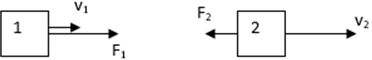
\includegraphics[scale=1]{../figs/VN10-2021-PH-TP0002-1.png}
		\end{center}
		Kết luận nào sau đây đúng?
		\begin{mcq}(2)
			\item $v_1$ tăng, $v_2$ giảm. 
			\item $v_1$ giảm, $v_2$ tăng. 
			\item $v_1$, $v_2$ cùng giảm. 
			\item $v_1$, $v_2$ cùng tăng. 
		\end{mcq}
	}
	
	\hideall
	{	\textbf{Đáp án: A.}
		
		$F_1$ cùng phương, cùng chiều với $v_1$ nên $v_1$ tăng.
		
		$F_2$ cùng phương, ngược chiều với $v_2$ nên $v_2$ giảm.
		
	}
	\item \mkstar{2}
	
	
	{Một vật chịu tác dụng của hai lực và đang chuyển động thẳng đều. Nhận xét nào sau đây là đúng?
		\begin{mcq}
			\item Hai lực tác dụng là hai lực cân bằng.
			\item Hai lực tác dụng có độ lớn khác nhau.
			\item Hai lực tác dụng có phương khác nhau.
			\item Hai lưc tác dụng có cùng chiều.
		\end{mcq}
	}
	
	\hideall
	{\textbf{Đáp án: A.}	
		
		
	}
	\item \mkstar{2}
	
	
	{Một xe đang chuyển động đều trên đường thì đột ngột dừng lại. Hành khách trên xe sẽ bị ngã về phía nào?
		
		\begin{mcq}(2)
			\item Ngã sang phải.	
			\item Ngã sang trái.
			\item Ngã về trước.	
			\item Ngã về sau.	
		\end{mcq}
		
	}
	
	\hideall
	{\textbf{Đáp án: C.}
		
	}
	\item \mkstar{2}
	
	
	{Khi ngồi trên xe ô tô thì hành khách bỗng thấy mình nghiêng sang trái. Nhận xét nào sau đây đúng?
		
		\begin{mcq}(2)
			\item Xe đột ngột tăng vận tốc.	
			\item Xe đột ngột giảm vận tốc.	
			\item Xe đột ngột rẽ sang phải.	
			\item Xe đột ngột rẽ sang trái.	
		\end{mcq}
		
	}
	
	\hideall
	{\textbf{Đáp án: C.}
		
	}
	\item \mkstar{2}
	
	
	{Trong các chuyển động sau, chuyển động nào là do quán tính?
		
		\begin{mcq}
			\item Hòn đá lăn từ trên núi xuống.	
			\item Xe máy chạy trên đường.	
			\item Lá rơi từ trên cao xuống.
			\item Xe đạp vẫn chạy dù thôi không đạp nữa.
		\end{mcq}
		
	}
	
	\hideall
	{\textbf{Đáp án: D.}
		
	}
	\item \mkstar{2}
	
	
	{Hai lực cân bằng là hai lực
		\begin{mcq}
			\item cùng điểm đặt, cùng phương, cùng chiều và cường độ bằng nhau.
			\item cùng điểm đặt, cùng phương, ngược chiều và cường độ bằng nhau.
			\item khác điểm đặt, cùng phương, cùng chiều và cường độ bằng nhau.
			\item khác điểm đặt, cùng phương, ngược chiều và cường độ bằng nhau.
		\end{mcq}
		
	}
	
	\hideall
	{\textbf{Đáp án: B.}
		
		Hai lực cân bằng là hai lực cùng điểm đặt, cùng phương, ngược chiều và cường độ bằng nhau.
	}
	\item \mkstar{2}
	
	
	{Một vật đang đứng yên trên mặt phẳng nằm ngang. Các lực cân bằng là
		
		\begin{mcq}
			\item trọng lực tác dụng lên vật và lực ma sát giữa vật với mặt bàn.	
			\item trong lực tác dụng lên vật và phản lực do mặt phẳng ngang tác dụng lên vật.
			\item trọng lực tác dụng lên vật và lực hấp dẫn do vật tác dụng lên Trái Đất.
			\item phản lực của mặt phẳng ngang và lực ma sát.	
		\end{mcq}
		
	}
	
	\hideall
	{\textbf{Đáp án: B.}
		
	}
	\item \mkstar{2}
	
	
	{Khi có lực tác dụng lên vật, mọi vật đều không thể thay đổi vận tốc một cách đột ngột được vì
		
		\begin{mcq}(4)
			\item ma sát.
			\item trọng lực.
			\item quán tính.	
			\item đàn hồi.
		\end{mcq}
		
	}
	
	\hideall
	{\textbf{Đáp án: C.}
		
	}
	\item \mkstar{2}
	
	
	{Chọn câu đúng nhất. Khi có lực tác dụng lên vật thì
		
		\begin{mcq}(2)
			\item vật chuyển động nhanh dần.	
			\item vật chuyển động chậm dần.
			\item vật biến dạng hoặc biến đổi chuyển động.	
			\item vật bay lên cao.	
		\end{mcq}
		
	}
	
	\hideall
	{\textbf{Đáp án: C.}
		
		
	}
	\item \mkstar{3}
	
	
	{Một quả bóng khối lượng $\SI{0.5}{kg}$. Trọng lượng của quả bóng là
		
		\begin{mcq}(4)
			\item $\SI{0.5}{N}$.	
			\item $\SI{5}{N}$.	
			\item $\SI{0.5}{kg}$.	
			\item $\SI{5}{kg}$.	
		\end{mcq}
		
	}
	
	\hideall
	{\textbf{Đáp án: B.}
		
		Trọng lượng vật: $P=10m = \SI{5}{N}$.
	}
	\item \mkstar{3}
	
	
	{Một quả bóng khối lượng $\SI{0.5}{kg}$. Lực căng dây treo quả bóng phải có độ lớn bao nhiêu để quả bóng nằm cân bằng?
		
		\begin{mcq}(2)
			\item $\SI{0.5}{N}$.	
			\item $\SI{5}{N}$.	
			\item lớn hơn $\SI{5}{N}$.	
			\item nhỏ hơn $\SI{0.5}{N}$.	
		\end{mcq}
		
	}
	
	\hideall
	{\textbf{Đáp án: C.}
		
		Để quả bóng nằm cân bằng thì $T=P=10m=\SI{5}{N}$.
	}

\item\mkstar{3}\\
{Cho hai lực khác phương có độ lớn bằng $\SI{9}{\newton}$ và $\SI{12}{\newton}$. Độ lớn của hợp lực có thể nhận giá trị nào sau đây?
	\begin{mcq}(4)
		\item $\SI{15}{\newton}$.
		\item $\SI{1}{\newton}$.
		\item $\SI{2}{\newton}$.
		\item $\SI{25}{\newton}$.
	\end{mcq}
}
\hideall{
\textbf{Đáp án: A.}
}

\item \mkstar{3}\\
{Một vật khối lượng $\SI{500}{\gram}$ chuyển động nhanh dần đều với vận tốc ban đầu $\SI{3}{\meter/\second}$. Sau thời gian $\SI{5}{\second}$, nó đi được quãng đường $\SI{24}{\meter}$. Biết vật luôn chịu tác dụng của lực kéo $\overrightarrow{F_k}$ có độ lớn không đổi và lực cản có độ lớn $F_c=\SI{5.64}{\newton}$ theo phương chuyển động. Độ lớn lực kéo là 
	\begin{mcq}(4)
		\item $\SI{4}{\newton}$.
		\item $\SI{6}{\newton}$.
		\item $\SI{1}{\newton}$.
		\item $\SI{5.5}{\newton}$.
	\end{mcq}

}
\hideall{
\textbf{Đáp án: B.}\\
Gia tốc của vật:
$$s=v_0t+\dfrac{1}{2}at^2\Rightarrow a=\SI{0.72}{\meter/\second^2}$$
Độ lớn lực kéo:
$$F_k=ma+F_c=\SI{6}{\newton}.$$
}

\item\mkstar{4}\\
{Chất điểm chịu tác dụng của lực có độ lớn là $F_1$ và $F_2=\SI{6}{\newton}$. Biết hai lực này hợp với nhau góc $\SI{150}{\degree}$ và hợp lực của chúng có giá trị nhỏ nhất. Giá trị của $F_1$ là 
	\begin{mcq}(4)
		\item $\SI{2}{\newton}$.
		\item $\xsi{3\sqrt{3}}{\newton}$.
		\item $\SI{3}{\newton}$.
		\item $\SI{5}{\newton}$.
	\end{mcq}

}
\hideall{
\textbf{Đáp án: B}\\
Ta có $F^2=F^2_1+F^2_2+2F_1F_2\cos\SI{150}{\degree}$
$$\Leftrightarrow F^2_1-6\sqrt{3}F_1+36-F^2=0\qquad (*)$$
Phương trình (*) là phương trình bậc 2 đối với ẩn $F_1$ có $\Delta =\left(6\sqrt{3}\right)^2-4\cdot\left(32-F^2\right)$.\\
Để phương trình (*) có nghiệm thì 
$$\Delta \ge 0 \Rightarrow F\ge \xsi{\sqrt{5}}{\newton}$$
Dấu "=" xảy ra khi $F_1=\xsi{3\sqrt{3}}{\newton}$.
}
	
\end{enumerate}
\section{Bài tập tự luận}
\begin{enumerate}[label=\bfseries Bài \arabic*:,leftmargin=1.5cm]
	\item \mkstar{2}
	
	
	{Hãy giải thích các hiện tượng sau và cho biết trong các hiện tượng này, ma sát có ích hay có hại?
		\begin{enumerate}
			\item Khi đi trên sàn gạch đá hoa mới lau dễ bị ngã;
			\item Ô tô đi vào chỗ bùn lầy, có khi bánh xe quay tít mà vẫn không thể thoát ra được;
			\item Giày đi lâu ngày bị mòn đế;
			\item Phải bôi nhựa thông vào dây cung ở cần kéo nhị (đàn cò).
		\end{enumerate}
	}
	
	\hideall
	{
		\begin{enumerate}
			\item Khi đi trên sàn gạch đá hoa mới lau dễ bị ngã;
			
			Sàn đá hoa trơn, khi có nước thì giảm độ ma sát giữa chân và sàn. Ma sát có ích, giúp người không bị ngã.
			
			\item Ô tô đi vào chỗ bùn lầy, có khi bánh xe quay tít mà vẫn không thể thoát ra được;
			
			Bánh xe không có ma sát với mặt đường, hoặc ma sát rất nhỏ không đủ để ô tô tiến lên. Ma sát có ích, giúp ô tô di chuyển được.
			
			\item Giày đi lâu ngày bị mòn đế;
			
			Giày ma sát nhiều với sàn nên bị mòn. Ma sát có hại vì làm mòn giày.
			
			\item Phải bôi nhựa thông vào dây cung ở cần kéo nhị (đàn cò).
			
			Bôi nhựa thông để tăng ma sát giữa dây cung và cần giúp đàn phát ra tiếng to hơn. Ma sát có ích vì giúp đàn phát ra tiếng to hơn.
		\end{enumerate}
	}

	\item \mkstar{2}
	
	
	{Vật $\SI{2}{kg}$ chuyển động thẳng đều trên mặt phẳng ngang bằng một lực kéo có độ lớn $\SI{0,8}{N}$. Lấy $g=\SI{10}{m/s}^2$. Tính hệ số ma sát trượt.
	}
	
	\hideall
	{
		Lực ma sát bằng lực kéo nên ta có biểu thức:
		
		$$F_\text{k} = F_\text{ms} \Rightarrow \mu = \dfrac{F_\text{k}}{mg} =\text{0,04}.$$
	}
	
		\item \mkstar{2}
	
	
	{ 
		Một xe bán tải khối lượng 2,5 tấn đang di chuyển trên cao tốc với tốc độ $\SI{90}{km/h}$. Các xe cần giữ khoảng cách an toàn so với xe chạy phía trước $\SI{70}{m}$. Khi xe đi trước có sự cố và dừng lại đột ngột. Hãy xác định lực cản tối thiểu để xe bán tải có thể dừng lại an toàn
		
	}
	
	\hideall
	{
		Ta có: $v = \SI{90}{km/h} = \SI{25}{m/s}$; $v_0 = 0$; $s = \SI{70}{m}$; $m = \text{2,5}\ \text{tấn} = \SI{2500}{kg}.$
		
		Gia tốc tối thiểu của xe là:
		
		$$a = \dfrac{v^2 - v_0^2}{2s} = \xsi{\dfrac{125}{28}}{m/s}^2.$$
		
		Lực tối thiểu để xe bán tải dừng lại an toàn
		
		$$F = ma \approx \SI{11160,7}{N}.$$
		
		
	}
	
	\item\mkstar{2}\\
	{Một người nhảy dù có khối lượng tổng cộng $\SI{100}{\kilogram}$. Trong thời gian đầu (khoảng vài giây) kể từ khi bắt đầu nhảy xuống, người này chưa mở dù và rơi dưới tác dụng của trọng lực. Khi người đó mở dù, lực tác dụng của dù lên người là $\SI{2000}{\newton}$ hướng lên.
		\begin{enumerate}[label=\alph*)]
			\item Biểu diễn các lực tác dụng lên người nhảy dù khi mở dù.
			\item Xác định hợp lực tác dụng lên người nhảy dù khi mở dù.
			\item Người sẽ chuyển động như thế nào kể từ khi mở dù?
		\end{enumerate}
	
}
\hideall{
\begin{enumerate}[label=\alph*)]
	\item 
	\begin{center}
		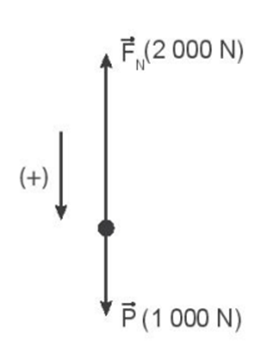
\includegraphics[width=0.3\linewidth]{../figs/VN10-2023-PH-TP0004-1}
	\end{center}
\item Hợp lực tác dụng lên người nhảy dù hướng lên và có độ lớn $F=\SI{1000}{\newton}$.
\item Khi chưa mở dù, người nhảy dù chuyển động nhanh dần đều dưới tác dụng của trọng lực (rơi tự do). Sau khi mở dù, người nhảy dù sẽ chuyển động chậm dần đều với gia tốc
$$a=\dfrac{P-F_N}{m}=\SI{-10}{\meter/\second^2}.$$
\end{enumerate}
}

\item\mkstar{3}\\
{Một vật khối lượng $\SI{2.5}{\kilogram}$ đang nằm yên trên mặt phẳng ngang thì chịu tác dụng của lực kéo $\SI{15}{\newton}$ theo phương ngang và bắt đầu chuyển động. Biết trong 1 phút đầu tiên sau khi chịu tác dụng lực, vật đi được $\SI{2700}{\meter}$. Coi lực cản tác dụng vào vật không đổi trong quá trình chuyển động. Xác định độ lớn của lực cản tác dụng vào vật.

}
\hideall{
Gia tốc của vật:
$$a=\dfrac{2s}{t^2}=\SI{1.5}{\meter/\second^2}$$
Lực cản tác dụng lên vật:
$$F_c=F_k-ma=\SI{11.25}{\newton}.$$

}
	
\item \mkstar{4}\\
{Một vật làm bằng sắt và một vật làm bằng hợp kim có cùng khối lượng được nhúng vào cùng một chất lỏng. Hỏi lực đẩy Archimedes tác dụng lên vật nào lớn hơn và lập tỉ số giữa hai lực đẩy Archimedes này? Biết khối lượng riêng của sắt và của hợp kim lần lượt là $\SI{7874}{\newton/\meter^3}$ và $\SI{6750}{\newton/\meter^3}$.

}
\hideall{
Theo giả thiết $m_s=m_{hk}\Rightarrow \dfrac{V_s}{V_{hk}}=\dfrac{\rho_{hk}}{\rho_s}=0,875$.\\
Ta có:
$$\dfrac{\left(F_A\right)_s}{\left(F_A\right)_{hk}}=\dfrac{V_s}{V_{hk}}=0,875.$$
}
\end{enumerate}